% 
%% Replace 'XX' with your paper number (assigned when you register abstract)
%% Replace 'NN' with actual number of pages. 

\documentclass[10pt,preprint,numbers]{sigplanconf}
%========================
%  Packages
%========================
\usepackage{times}
\usepackage{datetime}
\usepackage{url}
\usepackage{hyperref}
\usepackage{color}
\usepackage{graphicx}
\usepackage{algorithm}
\usepackage[noend]{algpseudocode}

%========================
%  Macros
%========================

\newcommand{\code}[1]{\textsf{\fontsize{9}{11}\selectfont #1}}

\newcommand{\inred}[1]{{\color{red}{#1}}}
\newcommand{\remove}[1]{}
\newcommand{\Idit}[1]{\inred{[Idit: #1]}}

\newcommand{\sys}{Pi\~na}

\newcommand{\tuple}[1]{\ensuremath{\langle \mbox{#1} \rangle}}



\conferenceinfo{SOSP'17}{October 29--31, 2017, Shanghai, China}
\copyrightyear{2017} 

% These only appear when the 'preprint' option is specified.
% Enabling these will cause the first page of the document to fail the 
% format check on HotCRP :-(
\titlebanner{Under submission to SOSP 2017 - do not cite or distribute}
\preprintfooter{Draft of {\currenttime}, \today{}}

% No date in title area.
\date{}

% Paper number and no. of pages as author
\authorinfo{Paper \textbf{\#XX}}{NN pages}

% Actual document begins below.
\begin{document}

\title{\sys: Persistent Key-Value Storage for Real-Time Analytics} 
\maketitle

\begin{abstract}

TBD

\end{abstract}

\section{Introduction}
%%%%%%%%%%%%%%%%%%%%%%%%%%%%%%%%%%%%%%%%%%%%%%%%%%%%%%%%%%%%%%%%%%%%%%%%%
\subsection{Motivation:  spatial locality in KV-storage}
% KV-storage workloads} 
%%%%%%%%%%%%%%%%%%%%%%%%%%%%%%%%%%%%%%%%%%%%%%%%%%%%%%%%%%%%%%%%%%%%%%%%%

% KV-stores are everywhere
Key-value stores (KV-stores) are widely used  by a broad range of applications and are projected
to continue to increase in popularity in years to come; market research  identifies them as the 
``driving factors'' of the NoSQL market, which is expected to garner \$4.2B by 2020~\cite{alliedmarketresearch}.

% In many applications, keys are composite
KV-stores provide a simple programming model. 
Data is an ordered collection of key-value pairs, and the API supports random writes, 
random reads, and range queries. 

A common design pattern is the use of \emph{composite} keys that represent an agglomerate of attributes.
Typically, the primary attribute (key prefix) %-- called the \emph{primary key} -- 
has a skewed distribution, and so   access via the composite key exhibits \emph{spatial locality}, as 
popular key prefixes result in popular key ranges~\cite{facebook-workloads}. 

One example of this arises in mobile analytics platforms, e.g., AppsFlyer~\cite{appsflyer}, Flurry~\cite{flurry}, 
and Google Firebase~\cite{firebase}. %~\cite{medium-mobile-analytics}.   
Such platforms %help mobile developers collect user activity data, analyze it, and optimize their app experience. They 
ingest massive streams of app event reports %(e.g., start, stop, or particular scenario within an app), 
in  real-time and provide a variety of insight queries into the data. For example, Flurry tracked events from  
1M+ apps across 2.6B user devices  in 2017~\cite{FlurryReport2017}. In order to offer per-app analytics efficiently,
such services aggregate data in KV-stores indexed by a composite key prefixed by a unique app 
id,  followed by a variety of other attributes (time, user id, device model, location, event type, etc.).
%
We examine a trace of almost $2$B  events captured from a production mobile analytics engine 
over half an hour.  
\Cref{fig:cdf} shows the access frequency distribution over the  $60$K app ids occurring in this stream. It follows a marked
heavy-tail pattern: 
%$10$\% of the apps cover over $99.5$\% of the events; 
$1$\% of the apps  cover $94$\% of the events, and fewer 
than $0.1$\% cover $70$\% of them. 

% This means the data is highly skewed and with a very long tail (not depicted in the figure).
%Table~\ref {table:popular} shows the cumulative probability of the top-$20$ popular applications, covering more than $50$\% of the events. 
%With application name as the primary dimension of a composite key this distribution induces high spatial locality.


\begin{figure}[tb]
\centering
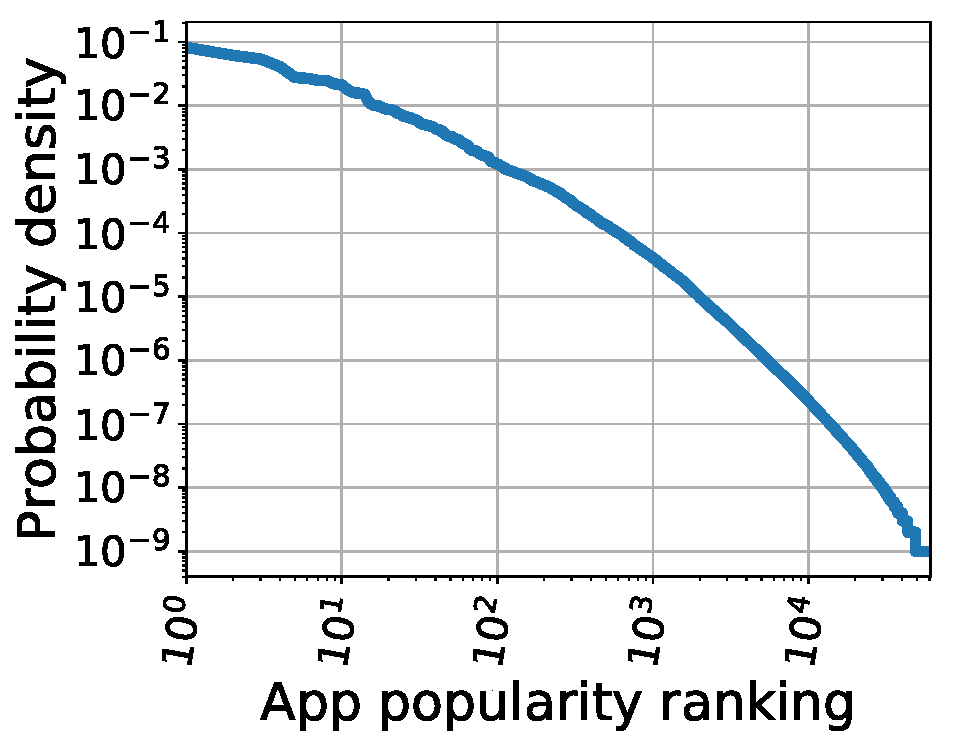
\includegraphics[width=0.6\columnwidth]{figs/app_names_loglog_line.pdf}
\caption{{Distribution of mobile app events by app id (log-log scale) in a production analytics feed (2B events).}}
\label{fig:cdf}
\end{figure}

Composite keys arise in many additional domains, including messaging and social networks~\cite{facebook-workloads}. 
For example, a backend Facebook Messenger query may retrieve the last 100 messages for a 
given user~\cite{Borthakur:2011:AHG:1989323.1989438}; %, where the primary key is user id. 
in Facebook's social network, a graph edge is indexed by a key consisting of two 
object ids and an association type~\cite{Armstrong:2013:LDB:2463676.2465296}.
%Note further that 
Spatial locality   also arises with simple (non-composite) keys, for example, when 
reverse  URL domains are used as keys for web  indexing~\cite{Cho:1998:ECT:297805.297835}. 

% Overfitting for Zipf 
The prevalence of skewed (e.g., Zipfian)  access  in real workloads is widely-recognized 
and reflected in standard benchmarks (e.g., YCSB~\cite{YCSB}). %  feature heavy-tailed key-access distributions like Zipf.
But these benchmarks fail to capture the spatial aspect of locality, which has gotten far less attention.
% Idit: removed below, too bold
%This, in turn, leads to storage systems being optimized for a skewed distribution on individual keys, % with no spatial locality,
%e.g., in partitioning data by  recent access time as opposed to by key range.
In this work, we make spatial locality a first-class consideration in KV-store design.
% which leads us to rethink the design principles underlying today's popular KV-stores.



%%%%%%%%%%%%%%%%%%%%%%%%%%%%%%%%%%%%%%%%%%%%%%%%%%%%%%%%%%%%%%%%%%%%%%%%%
\subsection{Spatial locality: the challenge}  
\label{ssec:B-tree-compare}
%%%%%%%%%%%%%%%%%%%%%%%%%%%%%%%%%%%%%%%%%%%%%%%%%%%%%%%%%%%%%%%%%%%%%%%%%



% LSM is the standard 
The de facto standard design for high-throughput KV-stores today is \emph{LSM} (log-structured merge) trees~\cite{DBLP:journals/acta/ONeilCGO96}. 
LSMs initially group writes  into files \emph{temporally} rather than by key-range. 
A background \emph{compaction} process later merge-sorts any number of files, grouping data by keys. 

% LSM is  not ideal for spatial locality  because of  temporal grouping 
This approach is not ideal for workloads with high spatial locality for two reasons. 
First,  popular key ranges are fragmented across many files. 
Second,  compaction  is costly in terms of  both performance 
(disk bandwidth) and \emph{write amplification}, namely the number of physical writes 
associated with a single application write. The latter is  particularly important in SSDs as it increases disk wear. 
The temporal grouping means that compaction is indiscriminate with respect to key popularity:  
Since new  files are always merged with old ones, 
 ``cold'' key ranges  continue to be repeatedly re-located by  compactions.  

% LSM is not the best when the entire working set fits in memory
Another shortcoming of LSM is that its temporal organization, while optimizing disk I/O,  penalizes in-memory operation. 
All updates -- including ones of popular keys -- are flushed to disk, even though persistence is assured via a separate \emph{write-ahead-log (WAL)}.
%Beyond increasing write amplification, this makes the flushed keys unavailable for fast read from memory,
%which is  wasteful if the system incorporates sufficient DRAM to hold most of the active working set. 
%The drop in DRAM prices (more than $6.6\times$ since 2010~\cite{dram-prices}) makes the latter scenario increasingly common.  

Yet  LSMs have supplanted the  traditional spatial data partitioning of B-trees for a reason~\cite{rocks-vs-inno}.
%A crucial challenge arising in spatially-organized  storage is how to persist all updates in a consistent way without sacrificing performance.
In  B-trees, each update induces random I/O  to a leaf, resulting in poor write performance.
Moreover, the need to preserve a consistent image of a leaf while it is being over-written induces high write amplification. 
$B^{\epsilon}$-trees~\cite{Brodal:2003:LBE:644108.644201} mitigate this cost using write buffers. % in internal tree nodes. 
However, this slows down lookups, which now have to search in unordered buffers, possibly on disk. 
% If the buffers reside on disk, the lookup time is unacceptably slow, whereas if they are in RAM then they have to be complemented by a separate persistence mechanism, with its own costs.  
%
LSMs, in contrast, achieve high write throughput by absorbing  writes in memory and periodically flushing them as 
sequential files to disk; they expedite reads by caching data in DRAM.

The resounding performance advantage of the LSM approach over B- and B$^{\epsilon}$-trees has been repeatedly demonstrated, 
e.g., in a recent  study of the Percona MySQL server using three storage engines -- RocksDB, TokuDB, and InnoDB --
based on LSM, a B$^{\epsilon}$-tree, and a B-tree, respectively~\cite{toku-rocks-inno}.
%
Another advantage of LSMs is that they readily ensure consistency under multi-threaded access -- in particular, atomic scans --   
via lock-free multi-versioning.
%This can be  tricky when a scan spans both memory-resident and disk-resident data.
In contrast, databases based on B- or  B$^\epsilon$-trees either use locks~\cite{innodblocking} 
or forgo scan consistency~\cite{tucana}.



\remove{
Obviously, we do not claim that spatial data partitioning is new; indeed, classical B-trees~\cite{DBLP:conf/sigmod/BayerM70,Comer79} 
 pre-date  LSM trees, and many B-tree variants~\cite{Brodal:2003:LBE:644108.644201,Bender15, Lehman:1981:ELC:319628.319663} have  emerged over the years. 
 However, it is important to note that these trees are  conceptual constructs rather than storage systems; 
 employing these concepts within a practical data store over a memory hierarchy 
 raises multiple challenges,  which perhaps explains their limited adoption in industrial KV-stores.
 A key challenge is what to persist when and in what format. 
 }
 
Our  goal is to 
%draw attention to the importance of spatial locality in today's KV-store workloads and to 
put forth a KV-store design alternative  suited for the 
spatial locality arising in today's  workloads, without forfeiting the benefits achieved by the LSM approach.




%%%%%%%%%%%%%%%%%%%%%%%%%%%%%%%%%%%%%%%%%%%%%%%%%%%%%%%%%%%%%%%%%%%%%%%%%
\subsection{Our contribution: \sys}
%%%%%%%%%%%%%%%%%%%%%%%%%%%%%%%%%%%%%%%%%%%%%%%%%%%%%%%%%%%%%%%%%%%%%%%%%

% Drum roll 
We present \sys, a high-throughput persistent KV-store geared towards spatial locality. 
\sys's  architecture (\cref{sec:principles}) combines a spatial data organization with LSM-like  batch I/O. 
The pillars of our design are large \emph{chunks} holding contiguous key ranges. 
\sys's chunks are not merely  a means to organize data on-disk (like nodes in a B-tree). They 
are also the basic units for read-write DRAM caching, I/O-batching, logging, and compaction. 
This approach is unique.
%Typical KV-stores rely on OS-managed page caches (whereas chunks consist of many pages)  
%supplemented by application-level caches. 
Typical KV-stores rely on finer-grain OS- and application-level page caches (whereas chunks consist of many pages) and employ a global WAL. 

\remove{
B-trees, e.g., InnoDB, use read-write page caches~\cite{InnoDB-Buffer-Pool}, however they fail to capture spatial locality 
because their cache granularity is too fine, which results in poor-performing near-random writes~\cite{toku-rocks-inno}.  
LSM's, e.g., RocksDB, use caches for the read path only~\cite{RocksDB-blockcache}. Their temporal structure optimizes write
performance in the short term but degrades it in the long term, due to compactions. Here too, 
spatial locality remains unexploited.}

Our novel chunk-based organization has several benefits. 
First, chunk caching is effective for spatially-local workloads.
Second, chunk-level logging eliminates the need to log each update in a system-level WAL, thus 
reducing write amplification and expediting crash-recovery. 
Finally, using the same data structure for both the read-path (as a cache) and the write-path
(as a log) allows us to perform \emph{in-memory compaction}, reducing write amplification even further.

% Downsides
The downside of spatial partitioning is that if the data lacks spatial locality and the active working set is big, 
chunk-level I/O batching is ineffective. Moreover, 
caching an entire chunk for a single popular key is wasteful. 
We mitigate the latter by adding a \emph{row cache} for read access to hot keys. Even so, 
our design is less optimal for mixed read/write workloads lacking spatial locality, for which the LSM approach may yield better performance.  

%To further expedite access in different scenarios, we incorporate a number of additional mechanisms: 
%a volatile index for direct access to chunks by key; Bloom filters to reduce reads from disk-resident chunks; and 

Our algorithm (\cref{sec:design}) is designed for high concurrency. 
%among threads running put, get, and scan operations, as well as background maintenance (compaction). 
It supports atomic scans using low-overhead multi-versioning, where versions are increased only by scans and not by updates. 
It ensures consistency and correct failure-recovery. 
%While the mechanisms we employ are all variants of ones appearing in the literature, their combination is novel and results in a high-performance storage system.

We implement \sys\ in  C++ (\cref{sec:impl}) and extensively evaluate it (\cref{sec:eval})
via three types of workloads: (1) a production trace collected from a large-scale mobile analytics platform; 
(2)  workloads with synthetically-generated composite keys exercising  standard YCSB scenarios~\cite{YCSB};
and (3)  YCSB's traditional benchmarks, which employ simple (non-composite) keys.  
%In all cases, 
We compare \sys\ to the recent (Oct 2018) release of RocksDB~\cite{RocksDB}, a mature industry-leading LSM KV-store. 
We  experimented with two additional open-source KV-stores, PebblesDB~\cite{PebblesDB}  and  
% PreconaFT/
TokuDB~\cite{TokuDB} (the only publicly-available $B^{\epsilon}$-tree-based 
KV-store); both performed significantly worse than  RocksDB and \sys, so we focus on RocksDB results. 
%so we do not discuss them further.
%\inred{across the entire YCSB benchmark suite.} %, which is in line with previous studies of PerconaFT~\cite{tucana}, so we excluded them from further tests. 
Our main findings are: 
\begin{enumerate} 
  %   \setlength{\itemindent}{-10pt}
\item \sys\/ is  better than RocksDB under high spatial  locality.  
For instance, on a 256GB production dataset, \sys\ ingests data $4.4\times$ faster than RocksDB %,  scans recent  data up to 27\% faster, 
and reduces write amplification by almost $4\times$. 
%And in large synthetic composite-key workloads, \sys\  improves over RocksDB's throughput by $24\% - 75\%$. 
\item \sys\/ significantly outperforms RocksDB whenever most of the working set fits in RAM, 
%For example, with synthetic composite keys and a memory-resident working set, \sys\  
accelerating scans by up to $3.5\times$, puts by up to $2.3\times$, and gets by up to $2\times$. 
\item \sys's performance is  comparable to RocksDB's in traditional YCSB workloads without spatial locality.
%while its write amplification is much smaller.
\item RocksDB outperforms \sys\ (by 20--25\%)  in mixed read/write workloads with large active working sets and no spatial locality, 
although \sys's write amplification remains $\sim2\times$ smaller than RocksDB's. 
%\item \sys\ has lower write amplification, especially on large datasets.
\end{enumerate}

% Benefits
Our results underscore the advantages of \sys's spatially-organized chunks:
(1) eliminating fragmentation of key ranges  yields better  performance under spatial locality; 
(2) keeping hot ranges in memory leads to better performance when most of the working set fits in RAM; and 
(3) in-memory chunk compaction saves disk flushes and reduces write volume.  
In addition, in-chunk logging allows quick recovery from crashes with no need to replay a WAL.


~\cref{sec:related}  surveys related work and~\cref{sec:conclusions} concludes this paper. 


\section{Related Work}
\label{sec:related}

LSM stores -- RocksDB, HyperLevelDB, LevelDB, cLSM, BLSM.

$\epsilon^+$-trees and implelentations like Tucana~\cite{tucana}.
% Btrfs does not seem relevant, the empahsis there is CoW instead of MVCC


\section{Design Princples}
\label{sec:principles}


\sys\ is a persistent key-value store supporting atomic \emph{put, get}, and  \emph{range scan} (or scan) operations. 
Scans are atomic in the sense that all values returned by a single scan belong to a consistent snapshot reflecting
the state of the data store at a unique point in time.

\remove{
\sys\ is geared for high-throughput analytics applications, which (1) perform many range scans; 
(2) strive to accommodate the entire working set in RAM (for performance), and yet require  (3)
persistence with fast recovery. 

We now detail the key requirements from \sys\ and the design choices we made in order to meet them.

\subsection{Requirements}

The key requirements from \sys\ are  the following:
}

Our Key design goals are the following:
\begin{enumerate}\itemsep0pt
\item \emph{Optimizing for spatial locality and atomic scans.}
 Many applications support multi-dimensional exploration of data, 
 which they realize in a KV-store using composite keys. This induce spatial locality.  
 \remove{For example, a typical  KV-map used by an application like Flurry Analytics~\cite{flurry} 
 summarizes mobile traffic statistics grouped by a combination of dimensions like  date,  user-id, and application-id.}
In addition, a query that retrieves data pertaining to a particular dimension thus needs to atomically 
retrieve the values pertaining to a range of keys. 
%To favor analytics queries, it is important to optimize such scans. 
 

\item \emph{High performance and low write amplification with memory-resident working sets.}
To sustain high throughput, key-value stores nowadays leverage increasing DRAM sizes where they can hold most of the 
active data set. We strive for maximum performance in this ``high performance'' case.  
In addition to performance, we seek to minimize disk writes in order to reduce disk wear.

\item \emph{Fast recovery.}
Because crashes are inevitable, the mean-time-to-recover from crashes should be kept short.
Like other popular KV-stores~\cite{RocksDB,leveldb,hbase}, \sys\ supports \emph{asynchronous} persistence, 
where put requests are buffered in memory and periodically persisted to disk in bulk. 
This approach significantly reduces the latency of put operations, which do not wait for their data to be persisted.
The downside of this approach is potential loss of recently written data upon crash. 
\remove{For example, 
if data is flushed to disk every $10$ seconds, then put operations executed in the last $10$ seconds before the crash 
may be undone. 

Nevertheless, \sys\ ensures 
}
It is required that \emph{data consistency} is preserved following recovery, in the sense that 
if some put is lost, all ensuing (and thus possibly dependent) puts are lost as well, and the recovery is to a well 
defined execution point some time before the crash.
 
\remove{
 \paragraph{Low write amplification.} 
 Minimizing disk writes is important not only for performance, but also for disk wear reduction.
}
\end{enumerate}

%\subsection{Design choices}

Given the aforementioned requirements, we make the following design choices in \sys:

\begin{enumerate}\itemsep0pt
\item \emph{Chunk-based organization.}
We organize data, both on-disk and in-memory,  in large chunks pertaining to  key ranges.  
%This enables efficient support of range scans, with  high cache locality and minimal loading of new memory pages. 
%Both the read and the write path go through chunks. 
Each chunk has a file representation called  \emph{funk} (file chunk), and may be cached in a  memory data structure called \emph{munk} (memory chunck).
This organization exploits spatial locality and is friendly to range scans.

We use a number of techniques to optimize in-memory  access, including partially sorting keys in each chunk and 
indexing munks. 
To expedite access to  keys whose chunks are only on-disk  (i.e., have no munks), 
individual popular keys are cached in a \emph{row cache}, 
and \emph{Bloom filters} are used to limit excessive access to disk. 

\item \emph{Infrequent disk compactions.}
As long as a chunk is cached (has a munk), its funk's organization does not have to be optimized since 
queries do not access it. Therefore, \sys\ infrequently performs reorganization (compaction) on such funks.
Conversely, when a funk holds cold data, its organization hardly deteriorates, and therefore compaction is not necessary.
Note that this is unlike LSM-trees, where all disk components are compacted, regardless of which keys reside in memory and whether 
keys are hot or cold. 

\item \emph{Multi-versioning for atomic scans.}
\sys\ employs multi-versioning along with
copy-on-write to keep data versions required by atomic scans. 
In other words, if a put attempts to overwrite a key  required by an active scan, then a new version is created alongside the 
existing one, whereas versions that are not needed by any scan are not retained. 
Thus, version management incurs a low overhead (as it occurs only on scans). 
%It also defines a simple rule for garbage collecting old versions.

\item \emph{In-funk WALs.}
\sys\ logs writes within funks and refrains from duplicating the updates  in a separate WAL. This reduces write amplification and expedites recovery times. 
\end{enumerate}


\section{\sys\ Design}
\label{sec:design}


The API of \sys\ is presented in Section~\ref{ssec:api}. 
Section~\ref{ssec:layout} then discusses \sys's data organization. 
%Detailed description of \sys's operations is given in Section~\ref{ssec:ops}.  
Atomic scans are discussed in Section~\ref{ssec:scans}, and 
the data structure's maintenance is discussed in Section~\ref{ssec:rebalance}.

\subsection{API and guarantees}
\label{ssec:api}

\sys\ is a persistent key-value store supporting \emph{put, get}, and atomic \emph{range scan} (or scan) operations. 
Scans are atomic in the sense that all values returned by a single scan belong to a consistent snapshot reflecting
the state of the data store at a unique point in time.

\Idit{More on API?}

\sys\ ensures \emph{durability} of all updates by writing updates to disk synchronously as part of the \emph{put} operation.

\subsection{Data organization}
\label{ssec:layout}

\begin{figure}[htb]
\centerline{
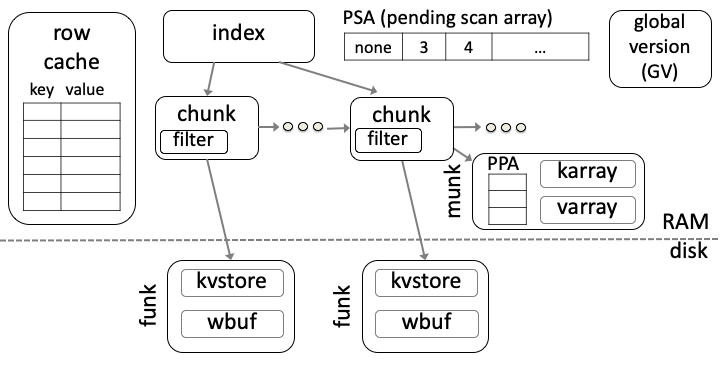
\includegraphics[width=0.9\columnwidth]{PiWi.png}
}
\caption{\sys\ data layout.}
\label{fig:layout}
\end{figure}

\paragraph{Chunk-based layout.}

\sys's data layout is depicted in Figure~\ref{fig:layout}.
Similarly to BTrees \Idit{and other disk-friendly data structures?}, 
\sys\ organizes data in fixed-size \emph{chunks}, each holding a contiguous key range.
This improves the efficiency of both disk access and memory access, in particular, for large range scans. 
At run-time, a list of all chunks is kept in RAM, where each chunk's data 
(consisting of keys in the corresponding range and values associated with them) 
is kept on disk (for persistence), and possibly in memory (for fast access). 

On disk, each chunk is associated with a \emph{file chunk}, or \emph{funk} --
a persistent data structure consisting of three files:  a value store \emph{vstore}, 
a compacted and sorted  key store \emph{kstore}, and a write buffer \emph{wbuf}. The vstore holds all the values associated with keys
in the chunk. When a funk is created, the kstore holds all the chunk's keys with pointers to corresponding values and the wbuf is empty.
New keys are subsequently appended to the unsorted wbuf, while new values are appended to the chunk's vstore.

This structure allows us to benefit from sorted searches on the kstore, and at the same time
allows for updating chunks without re-writing existing data, thus minimizing write amplification.
As a funk's wbuf grows, however, searching becomes inefficient   and  
the funk is no longer compact, i.e., it may contain redundant (over-written keys).
Therefore, once the wbuf exceeds a certain threshold, we reorganize the funk.

Since updates to disk are executed synchronously,  the data store reflecting all completed put operations 
can be consistently recovered from the on-disk funks at any time. \Idit{Need to discuss recovery somewhere.}

A subset of the chunks is also cached in memory to allow fast access, where each cached chunk is associated with a
\emph{memory chunk (munk)}  data structure. 
Munks are volatile and can be removed and recreated from funks at any time.
Thus, multiple \emph{generations} of munks may exist for a chunk throughout its life time.


At run-time, \sys\ holds in memory a linked list of chunk objects as well as 
%representing all funks in the data store. Chunks are also indexed in-memory for fast access by key using 
a \emph{chunk index}, which is a sorted map from keys to chunks (e.g., a sorted array, skip list, or search tree).
Note that since chunk objects do not hold actual keys and values, they are significantly smaller than munks and funks. 
\inred{A typical chunk object is smaller than 1KB, whereas the size of a funk or munk that holds 10K to 100K keys 
ranges between 1M to 100M depending on the data size. A typical \sys\ node holds thousands of chunks, with 
all chunk objects in memory in addition to hundreds of munks.} 


A munk consists of two arrays -- karray and varray -- where the karray implements a sorted linked list of the chunk's keys. 
When a munk is created, its karray is sorted by key, so each cell's successor in the linked list is the ensuing cell in the array.
As new keys are added, they create bypasses in the linked list and karray is no longer sorted.
Key removals, in turn, leave obsolete values in the karrray, so it is no longer compacted.

As key-value pairs are added, overwritten, and removed, munks and funks need to undergo reorganization. This includes  
\emph{compaction} to deallocate removed and overwritten data, 
\emph{sorting} keys to make searches more efficient,  and
\emph{splitting} overflowing chunks.
\remove{, and \emph{merging} under-utilized ones.}
All reorganizations are performed by \sys's \emph{rebalance} operation.
If the chunk has a munk, then rebalance compacts and sorts the munk in-memory by creating a new 
(compacted and sorted) munk instead of the existing one. 
Funks of uncached chunks are also compacted by replacing them with new funks, albeit less frequently.
Splits  create new chunks as well as new  funks (and possibly munks) associated with them.


\paragraph{Data structures.}

In addition to the chunk list and chunk index, \sys\ keeps a \emph{global version (GV)} for supporting atomic snapshot scans,
as described below; it tracks active scans in a \emph{pending scan array (PSA)} for garbage collection purposes (old 
versions not needed by any active scan can be reclaimed).

The chunk data structure is given in Algorithm~\ref{alg:chunk}. 
The first field is its status, which is explained  below. 
It next holds a pointer to the appropriate funk, and, if applicable, also munk, as well as a pointer to the next 
chunk in the chunk linked list.
It further keeps the generation number of its latest munk and a per-generation sequence number,
which, in case there is an active munk, is the index of the next free cell in the munk's karray and varray.


\begin{algorithm}[htb]
\begin{algorithmic}
\State status \Comment  baby, child, active, asleep, or aged
\State ptr funk \Comment funk disk address
\State ptr munk \Comment munk memory pointer
\State ptr next \Comment next chunk in linked list
\State int gen \Comment munk generation
\State int seq \Comment sequence number in current generation 
\State asymmetric lock rebalanceLock \Comment r/w lock 
\State lock funkChangeLock \Comment acquired with try\_lock 
\State PPA[threads] \Comment pending put array
\end{algorithmic}
\caption{Chunk data structure.}
\label{alg:chunk}
\end{algorithm}


The chunk additionally includes locks and data structures to synchronize concurrent access by multiple threads.
The replacement of a chunk (due to a split) or of a funk or munk associated with a given chunk 
must be executed atomically, and moreover, must be synchronized with concurrent puts. 
This is controlled by the chunk's rebalanceLock, which is held for short time periods
during chunk/funk/munk replacements.  It is a shared/exclusive lock (r/w lock), acquired in shared mode 
by put operations and in exclusive mode by rebalance. Gets and scans do not need to acquire the lock at all,
and are completely wait-free.

To minimize I/O, we allow at most one thread to rebalance a funk at a given time; this is controlled by 
the  funkChangeLock. This lock is used at a coarse granularity -- it is held throughout the creation of the new funk. 
It is acquired using a try\_lock call, and threads that fail to acquire it do not retry, but instead wait for the winning thread 
to complete the funk's creation.
Finally, the chunk holds a data structure called PPA for synchronizing  puts with concurrent scans, as explained in the next section. 


\subsection{Supporting atomic scans}
\label{ssec:scans}


\paragraph{Multi-versioning.}

We support atomic scans via multi-versioning using a system-wide global version, GV. 
A scan operation creates a \emph{snapshot} associated with GV's current value by incrementing GV, 
which signals to ensuing put operations that they must not overwrite values associated with 
smaller versions than the new GV value.
This resembles a \emph{copy-on-write (CoW)} approach, which virtually creates a snapshot by 
indicating that data pertaining to the snapshot should not be modified in place.  

To allow garbage collection of old versions, \sys\  maintains 
a pending scan array, PSA, with one entry per active thread, tracking snapshot times of ongoing scans.
The compaction process that runs as part of rebalance removes versions that are no longer required for any  
scan in the PSA. Specifically, for each key, it removes all but the last version that is smaller than the minimal
PSA entry. 

For linearizing (i.e., determining an order on) updates, we associate each key-value pair written to the data store 
with a unique-per-key identifier.
This identifier is a tuple $\langle$ver, gen, seq$\rangle$, where \emph{ver} is  the version read from GV 
(recall that GV is only incremented upon scans and hence might remain unchanged across multiple puts),
\emph{gen} is the generation of the target chunk's last created munk  (which may or may not still exist), 
and seq is the running sequence number of values inserted to the chunk in the current generation.

\paragraph{Concurrent puts and scans.}

A put operation obtains a version number from GV, and a scan begins by fetching and incrementing GV.
If a put obtains its version before a scan, then the new value must be included in the scan's snapshot. 
However, because the put's access to the GV and the insertion of the new value to the chunk do not occur atomically,
a subtle race may arise. Consider a put operation that obtains version $7$ from GV and then stalls before
inserting the value to the chunk, while a scan obtains version $7$ and increments GV to $8$. The scan then proceeds 
to read the appropriate chunk and does not find the new value although it should be included in its snapshot.

To remedy this, we rely on a mechanism previously proposed in~\cite{kiwi} for synchronizing puts and scans in an in-memory map.  
The idea is to have scans ``help'' puts obtain a version, and to make the inserted key-value pair visible the moment it has a version.
The per-chunk PPA is used to synchronize pending puts  with ongoing scans. 
The PPA holds an entry for every active inserting thread.
A put operation first registers itself in the appropriate chunk's PPA entry with the key and value it intends to add.
It thens reads GV, and attempts to set the version field in its PPA entry to the read version using an atomic 
compare-and-swap (CAS) instruction. A scan, in turn, scans the PPA in addition to the chunk's data (karray 
or kstore). If it finds a value associated with a version, it considers it to have been inserted (and returns it if the version is
the highest version for this key that does not exceed its scan time). If it encounters a value without a version, the scan helps the put
assign a version, also by attempting to CAS the PPA's version field to the current value of GV.
For symmetry, get operations synchronize with puts the same way that scans do. 

\subsection{Reorganization}
\label{ssec:rebalance}

\paragraph{Synchronizing puts and rebalances.}

Rebalance is used to improve data organization in a chunk's funk or munk by removing old versions that are no longer needed for scans, 
removing deleted items, and sorting all the keys in the chunk. 
It can be invoked by any thread, either one attempting to access the chunk (typically for put) or a dedicated background thread.

In case a chunk has a munk, rebalance reorganizes only  the munk, since all searches are served by it. In case the chunk has no munk, the funk is reorganized. Reorganization involves creating a new funk or munk 
to replace the  current one.  In some cases, the chunk itself is split, creating new funks (and munks if applicable). We first discuss 
rebalances that do not involve splits; we revisit splits below.

A munk rebalance begins by obtaining the rebalanceLock in exclusive mode. Since puts acquire the lock in shared mode,
the lock is acquired when there are no active puts in the chunk, and blocks new puts that attempt to write to the same chunk. 
\remove{
%It also changes the chunk status to asleep, indicating that it is now immutable.
Since there might be active put threads at the time the chunk becomes immutable, the rebalance operation
needs to either take them into account or prevent them from proceeding. To this end, it uses the PPA. 
For each active put thread in the chunk, if the thread's PPA entry includes a value and a version, they
are copied into the new funk or munk. Otherwise, scan uses CAS to set the PPA version to ``asleep'', 
preventing the put from setting a version. 
}
When the new munk is ready, the rebalance process replaces the munk pointer in the chunk, releases rebalanceLock, and re-activates the chunk.
%A put operation that finds the target chunk immutable or its PPA version asleep waits on  rebalanceLock
%for rebalance to complete and then re-attempts the put. 

Since funk reorganization may take a long time, we allow the chunk to be active while the new funk is created,
and then make it immutable (as during munk rebalances) for a short time. In order to avoid redundant I/O, 
we use the funkChangeLock to ensure that only one thread is working to create a new funk.  Once that thread
completes, it acquires the rebalanceLock in exclusive mode.
It then copies to the new chunk any new items added to wbuf in the old chunk before it became immutable. 
When this is done, it replaces the funk pointer in the chunk, releases the lock, and re-activates the chunk.

\paragraph{Splits and chunk life cycle.}

As noted above, as a result of a rebalance operation, a chunk can undergo three types of changes: munk rebalance, funk rebalance
(when a munk does not exist), and split. The latter affects the chunk object as well as the munk (if exists) and the funk.

In case of a munk rebalance, the chunk is immutable throughout the rebalance operation.
%, and put operations targeting that chunk must wait or help rebalance to complete. 
In this simple case, the chunk's status changes to \emph{asleep} (indicating that it is immutable)
when rebalance begins, and changes back to \emph{active} when rebalance ends. 
Note that the asleep status is tantamount to the rebalanceLock being held in exclusive mode.

Since funk rebalance involves I/O, it may take a long time, and so we  refrain from sleeping for its entire 
duration. In this case, the chunk becomes asleep after most of the funk is populated, and 
changes back to active after we 
migrate the wbuf's new tail to the new chunk and swing the funk pointer in the chunk.


\begin{figure}[htb]
\centerline{
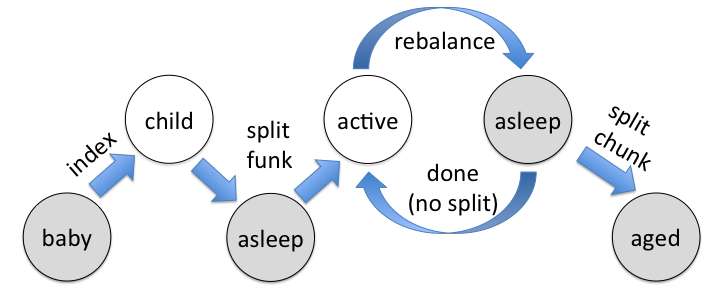
\includegraphics[width=\columnwidth]{state-diagram.png}
}
\caption{Chunk lifecycle; immutable states are grey and mutable ones are white.
Chunk splits  create new chunks in immutable \emph{baby} status, which changes to the mutable \emph{child} state once they 
are indexed. When the appropriate funks are created, the chunks become \emph{active}. All rebalance operations go through an 
\emph{asleep} state when the chunk is immutable.}
\label{fig:status}
\end{figure}

In the third case, the chunk is asleep when we create two new chunks to replace it. 
If the chunk has a munk, we split the munk (by creating two new munks) and update the appropriate pointers in the new chunks.  
Since creating new funks again involves I/O, we do not wish to keep the new chunks immutable for the duration of this process,
and allow funk creation to proceed in the background while the two new chunks still point to the same old funk. 

After we replace the old chunk in the list with the two new ones, 
the old chunk is still accessible via the chunk index (even though it is no longer in the list). 
The new chunks are therefore created in \emph{baby} status, indicating that they are still immutable. 
Once the new chunks are indexed, the old chunk is \emph{aged}, and the new chunks can become mutable.
At this point, we change their status to \emph{child}, indicating that they are no longer immutable, but share a funk with another chunk,
and so should not be rebalanced. Once the funk split completes, we put the chunks to sleep in order
to complete the funk switch and then change their  status  to active. 
The chunk's life-cycle is depicted in Figure~\ref{fig:status}.



\remove{
\subsection{\sys\ operations}
\label{ssec:ops}

\inred{Consider if we want full pseudocode}
}











\section{Evaulation}
\label{sec:eval}

To drive the benchmarks, we use the 
YCSB framework in C++\footnote{\url{https://github.com/basicthinker/YCSB-C}}  

We compare \sys\ to 
\begin{enumerate}
\item
LevelDB\footnote{\url{http://leveldb.org/}}
\item
RocksDB\footnote{\url{http://rocksdb.org/}}
\item
RocksDB with cLSM extensions\footnote{\url{https://github.com/guyg8/rocksdb}}
\end{enumerate}
All three systems are configured to provided persistence, namely, no data loss, by using their synchronous logging mode.
In addition, we deploy a single partition in each of the systems in order to provide consistent scans across the entire data store.

We do not compare with Tucana~\cite{tucana} as its code has not been available; moreover, it does not support the persistency and consistency guarantees that \sys\ provides. 


\section{Conclusions}
\label{sec:conclusions}
\sys\ rocks.

\bibliographystyle{acm}
 \bibliography{ref}

\end{document}
